\documentclass[11pt, openright]{book}

    % Cover Variables
    \newcommand{\ctitle}{MODULATION DELTA}
    \newcommand{\cautor}{Lucas Lescure - Eva Maturana}
    \newcommand{\ctoptitle}{}

    % Header Variables
        \newcommand{\headRE}{\emph{\thepage}}
        \newcommand{\headLE}{\emph{\thesubsection. \rightmark}}
        \newcommand{\footRE}{}
        \newcommand{\footLE}{}

    % TOC Variables
        \newcommand{\toctitle}{Table of Content}
        \newcommand{\tocchapter}{Chapter}
        \newcommand{\toccount}{3}
  
    % Chapter Variables
        \newcommand{\chvar}{Chapter -}

\usepackage[a4paper, total={16cm, 22.125cm}]{geometry}

% Page Style
\usepackage[]{environ}
% Cover Page 
\usepackage{tikz}
\makeatletter
\def\parsecomma#1,#2\endparsecomma{\def\page@x{#1}\def\page@y{#2}}
\tikzdeclarecoordinatesystem{page}{
    \parsecomma#1\endparsecomma
    \pgfpointanchor{current page}{north east}
    % Save the upper right corner
    \pgf@xc=\pgf@x%
    \pgf@yc=\pgf@y%
    % save the lower left corner
    \pgfpointanchor{current page}{south west}
    \pgf@xb=\pgf@x%
    \pgf@yb=\pgf@y%
    % Transform to the correct placement
    \pgfmathparse{(\pgf@xc-\pgf@xb)/2.*\page@x+(\pgf@xc+\pgf@xb)/2.}
    \expandafter\pgf@x\expandafter=\pgfmathresult pt
    \pgfmathparse{(\pgf@yc-\pgf@yb)/2.*\page@y+(\pgf@yc+\pgf@yb)/2.}
    \expandafter\pgf@y\expandafter=\pgfmathresult pt
}
\makeatother


% Object formatting
\usepackage[12pt]{moresize}
\usepackage[]{anyfontsize}
\usepackage{titlesec}
\usepackage{import}
\usepackage{floatrow}
\usepackage{enumitem}
\usepackage{changepage}
\usepackage[normalem]{ulem}
\usepackage{array}
\newcommand{\ul}[1]{\underline{#1}}

\usepackage[]{chngcntr}
\usepackage{ifthen}
\ifthenelse{\figcountdepth > 1}
  {\counterwithin{figure}{section}\counterwithin{table}{section}}
  {}

\usepackage[format=plain, labelfont=it, textfont=it]{caption}
\makeatletter
\def\@makecaption#1#2{%
    \vskip\abovecaptionskip
    \sbox\@tempboxa{\textit{#1.} #2}

       
   

    \ifdim \wd\@tempboxa >\hsize
        #1. #2\par
    \else
        \global \@minipagefalse
        \hb@xt@\hsize{\hfil\box\@tempboxa\hfil}
    \fi
    \vskip\belowcaptionskip}
\makeatother

\DeclareCaptionFormat{underline}{\uline{#1#2#3}\par}

% Sections
\titleformat{\section}{\fontsize{16}{19.2}\bfseries}{\thesection.}{0.25em}{}
\titleformat{\subsection}{\fontsize{14}{16.8}\bfseries}{\tab\thesubsection.}{0.25em}{}
\titleformat{\subsubsection}{\fontsize{10}{12}}{\uline{\thesubsubsection)\enspace}}{0em}{\uline}





% Geometry

% Typewritting

\setlength{\parskip}{1em}
\setlength{\parindent}{0em}


\newenvironment{items}[3][0pt]
{\def\closesep{#3}
    \vspace{#2}
    \begin{itemize}
        \setlength{\itemsep}{#1}
        \setlength{\topsep}{0pt}
        \setlength{\partopsep}{0pt}}
        {\end{itemize}
    \vspace{\closesep}}

\newenvironment{enum}[3][0pt]
{\defclosesep{#3}
    \vspace{#2}
    \begin{enumerate}
        \setlength{\itemsep}{#1}
        \setlength{\topsep}{0pt}
        \setlength{\partopsep}{0pt}}
        {\end{enumerate}
    \vspace{\closesep}}

\newenvironment{eq}[2]
{\def\closesep{#2}
    \vspace{#1}
    \begin{align*}}
        {\end{align*}
    \vspace{\closesep}}

\newenvironment{lfeq}[2]
{\def\closesep{#2}
    \vspace{#1}
    \begin{flalign*}}
        {\end{flalign*}
    \vspace{\closesep}}
% List Formatting


\NewEnviron{dent}[1]{
    \vspace{-10pt}
    \begin{adjustwidth}{7mm}{}
        \uline{#1}\hspace{2mm}
        \BODY
    \end{adjustwidth}
    \vspace{-10pt}
}


\usepackage[framemethod=tikz]{mdframed}
\newcounter{count_theorem}[section]\setcounter{count_theorem}{0}
\newcommand{\thetheorem}{\arabic{count_theorem}}

\newcounter{count_exercise}[section]\setcounter{count_exercise}{0}
\newcommand{\theexercise}{\arabic{count_exercise}}


\newenvironment{theorem}[1][]{
    \refstepcounter{count_theorem}
    \mdfsetup{
        linecolor=red!30,
        innerbottommargin=10pt,
        linewidth=2pt,
        topline=false,
        bottomline=false,
        rightline=false,
        shadow=true,
        shadowsize=4.5pt,
        frametitlerule=false,
        apptotikzsetting={
                \tikzset{
                    mdfbackground/.append style={
                            left color=red!8,right color=red!3
                        }
                }
            }
    }
    \begin{mdframed}[]\relax
        \ifstrempty{#1}
        {\textbf{Theorem~\thetheorem.} }
        {\textbf{Theorem~\thetheorem.~#1} }
        }
        {\end{mdframed}\vspace{-10pt}
}

\newenvironment{note}{
    \mdfsetup{innertopmargin=5pt,
        linecolor=gray!30,
        linewidth=2pt,
        topline=false,
        bottomline=false,
        rightline=false,
        frametitleaboveskip=0pt,
        shadow=false,
        shadowsize=4pt,
        frametitlerule=false,
        apptotikzsetting={
                \tikzset{
                    mdfbackground/.append style={
                            left color=gray!8,right color=gray!3
                        }
                }
            }
    }
    \begin{mdframed}[]\relax
        \textbf{Note. }
        }
        {\end{mdframed}\vspace{-10pt}
}

\newenvironment{example}{
    \mdfsetup{innertopmargin=5pt,
        linecolor=green!30,
        linewidth=2pt,
        topline=false,
        bottomline=false,
        rightline=false,
        frametitleaboveskip=0pt,
        shadow=false,
        shadowsize=4pt,
        frametitlerule=false,
        apptotikzsetting={
                \tikzset{
                    mdfbackground/.append style={
                            left color=green!7,right color=green!2
                        },
                    mdfframetitlebackground/.append style={
                            left color=green!7,right color=green!2
                        }
                }
            }
    }
    \begin{mdframed}[]\relax
        \textbf{Example. }
        }
        {\end{mdframed}\vspace{-10pt}
}


\usetikzlibrary{calc,arrows}

\tikzset{
    excursus arrow/.style={%
            line width=2pt,
            draw=gray!40,
            rounded corners=2ex,
        },
    excursus head/.style={
            fill=white,
            font=\bfseries\sffamily,
            text=gray!80,
            anchor=base west,
        },
    excursus line/.style={%
            line width=2pt,
            draw=gray!40,
            rounded corners=2ex,
        }
}

\newenvironment{exercise}[1][]{%
    \refstepcounter{count_exercise}
    \mdfsetup{
        singleextra={
                \path let \p1=(P), \p2=(O) in (\x2,\y1) coordinate (Q);
                \path let \p1=(Q), \p2=(O) in (\x1,{(\y1-\y2)/2}) coordinate (M);
                \path [excursus line] ($(O)+(5em,0ex)$) -| (M) |- ($(Q)+(20em,0ex)$);
                \node [excursus head] at ($(Q)+(2.5em,-0.75pt)$) {\ifstrempty{#1}{Exercise \theexercise}{Exercise \theexercise:~#1}};},
        firstextra={
                \path let \p1=(P), \p2=(O) in (\x2,\y1) coordinate (Q);
                \path [excursus arrow,-to] (O) |- ($(Q)+(12em,0ex)$) .. controls +(0:16em) and +(185:6em) .. ++(23em,2ex);},
        middlelinewidth=2.5em,middlelinecolor=white,
        hidealllines=true,topline=true,
        innertopmargin=0.5ex,
        innerbottommargin=2.5ex,
        innerrightmargin=2pt,
        innerleftmargin=2ex,
        skipabove=0.87\baselineskip,
        skipbelow=0.62\baselineskip,
    }
    \begin{mdframed}[]\relax}
        {\end{mdframed}\vspace{-10pt}
}

% Functions and Data Plotting
\usepackage{subfig,wrapfig,adjustbox,multirow}


% Plotting Style
\usepackage{graphicx,pgfplots}
\usetikzlibrary{arrows}
\usetikzlibrary {patterns,patterns.meta}
\usepgfplotslibrary{fillbetween}
\pgfplotsset{compat=1.18}

\usepgfplotslibrary{units}
% Logarithmic Scale
\pgfplotsset{
    log x ticks with fixed point/.style={
            xticklabel={
                    \pgfkeys{/pgf/fpu=true}
                    \pgfmathparse{exp(\tick)}%
                    \pgfmathprintnumber[fixed relative, precision=3]{\pgfmathresult}
                    \pgfkeys{/pgf/fpu=false}
                }
        }
}


% Mathematics

% Formatting
\usepackage{amsmath}
\usepackage{esvect}
\usepackage{amsfonts}
\usepackage{tasks,environ}
\usepackage{xargs}
\usepackage{esint}
\usepackage[]{listings}


\usepackage[english]{babel}
\usepackage{amsthm}
%\newtheorem{theorem}{Theorem}
%\newtheorem{proof}{Proof}



%Custom Shortcuts
\newcommand{\eqi}{\Leftrightarrow}
\newcommand{\lr}[1]{\left( #1 \right)}
\newcommand{\limit}[1]{\displaystyle{\lim_{#1}}}
\newcommand{\tab}{\hspace*{7mm}}
\newcommand{\ds}[1]{\displaystyle{#1}}
\newcommand{\floor}[1]{\lfloor #1 \rfloor}
\newcommand{\R}{\mathbb{R}}
\newcommand{\N}{\mathbb{N}}
\newcommand{\Z}{\mathbb{Z}}
\newcommand{\C}{\mathbb{C}}
\newcommand{\K}{\mathbb{K}}
\newcommand{\F}{\mathcal{F}}
\newcommand{\M}{\mathcal{M}}
\renewcommand{\l}{\lambda}
\newcommand{\seg}[1]{\overline{\rm {#1}}}
\newcommand{\Int}{\int\limits}
\newcommand{\ex}{\tab \uline{Example :}\hspace{0.2cm} }
\newcommand{\vard}{\partial}
\newcommand{\Q}{\mathcal{Q}}
\newcommand{\Vect}{\operatorname{Vect}}
\newcommand{\rg}{\operatorname{rg}}
\renewcommand{\dim}{\operatorname{dim}}
\renewcommand{\Re}{\operatorname{Re}}
\renewcommand{\Im}{\operatorname{Im}}
\renewcommand{\P}{\mathcal{P}}
\newcommand{\blr}[1]{\left\{#1\right\}}
\newcommand{\linecenter}[1]{\par\vspace{2mm} \centerline{#1}\par\vspace{-2mm}}
\newcommand{\dd}{\textrm{d}}
\newcommand{\supp}{\operatorname{Supp}}
\renewcommand{\vec}{\overrightarrow}
\renewcommand{\epsilon}{\varepsilon}

% Matrix Configurations

\makeatletter
\renewcommand*\env@matrix[1][*\c@MaxMatrixCols c]{%
    \hskip -\arraycolsep
    \let\@ifnextchar\new@ifnextchar
    \array{#1}}
\makeatother


% Colors
\usepackage{xcolor}
\newcommand{\blu}{\color{blue}}
\newcommand{\Red}{\color{red}}
\newcommand{\blac}{\color{black}}

\newcommand{\red}[1]{\textcolor{red}{#1}}

\usepackage{xcolor,xspace}
\usepackage{breqn}


% Headings  
\usepackage[Glenn]{fncychap}
\ChNumVar{\fontsize{40}{42}}
\ChTitleVar{\Large\sc}
\ChNameVar{\Large\sc}
\setlength\headheight{14.5pt}
\renewcommand\FmN[1]{\chvar}



\usepackage{fancyhdr}
\usepackage{ragged2e}

% Header & Footers
\renewcommand{\chaptermark}[1]{\markboth{#1}{#1}}
\renewcommand{\sectionmark}[1]{
    \markright{ #1}
}
\pagestyle{fancy}
\fancyhf{}
\fancyhead[LE,RO]{\headLE}
\fancyhead[RE,LO]{\headRE}
\fancyfoot[LE,RO]{\footLE}
\fancyfoot[RE,LO]{\footRE}
\renewcommand{\headrulewidth}{0.5pt}
\fancyheadoffset{1cm}

\fancypagestyle{plain}{%
    \fancyhf{} % clear all header and footer fields
    \fancyfoot[LE, RO]{\footLE}
    \renewcommand{\headrulewidth}{0pt}
    \renewcommand{\footrulewidth}{0pt}}


\fancypagestyle{nohead}{%
    \fancyhf{} % clear all header 
    \fancyfoot[LE, RO]{\footLE}
    \fancyfoot[LO, RE]{\footRE}}

    \fancypagestyle{head}{%
    \fancyhf{} % clear all header 
    \fancyhead[LE,RO]{\headLE}
\fancyhead[RE,LO]{\headRE}
\renewcommand{\headrulewidth}{0.5pt}
\fancyheadoffset{1cm}
    }


\fancypagestyle{bib}{%
    \fancyhf{} % clear all header and footer fields
    \fancyhead[CE, CO]{}
    \fancyfoot[LE, RO]{\footLE}
    \fancyfoot[LO, RE]{Bibliographie}}

% Table of Contents

\renewcommand*\thechapter{\arabic{chapter}} %Usually Roman
\renewcommand*\thesection{\arabic{section}}
\renewcommand*\thesubsubsection{\thesubsection.\alph{subsubsection}}
\makeatletter
\@removefromreset{section}{chapter}
\makeatother


% Table of Contents

\usepackage{titletoc}
\usepackage{ erewhon,cabin}
\usepackage[linktoc=all]{hyperref}
\renewcommand*\contentsname{\centerline{\toctitle}}

\setcounter{secnumdepth}{3}
\setcounter{tocdepth}{\toccount}

\usepackage[subfigure]{tocloft}
\setlength\cftparskip{0pt}

\usepackage{etoolbox}
\makeatletter
\pretocmd{\chapter}{\addtocontents{toc}{\protect\addvspace{5\p@}}}{}{}
\pretocmd{\section}{\addtocontents{toc}{\protect\addvspace{-10\p@}}}{}{}
\pretocmd{\subsection}{\addtocontents{toc}{\protect\addvspace{1\p@}}}{}{}
\makeatother


% Chapter Style
\titlecontents{chapter}
[11em]
{\bigskip}
{\bfseries\textsc\tocchapter~\textsc\thecontentslabel : \textsc}
{\hspace*{-5.5em}\textbf}
{\titlerule*[1pc]{ }}[\smallskip]

% Section Style
\titlecontents{section}
[0em] % i
{\bigskip\bfseries}
{\fontsize{11}{13.2}\bfseries\uline{\thecontentslabel.\enspace}\uline}
{\hspace*{-4em}\textbf}
{\hspace{0.5pt}\uline{\hspace*{\fill}}\contentspage}

% Subsection Style
\titlecontents{subsection}
[2em] % i
{\smallskip\bfseries}
{\fontsize{10}{12}\bfseries\thecontentslabel.\enspace}
{\hspace*{-4em}}
{\titlerule*[0.5pc]{.}\contentspage}

% Subsubsection Style
\titlecontents{subsubsection}
[4em] % i
{\smallskip}
{\fontsize{10}{12}\thecontentslabel)\enspace}
{\hspace*{-4em}}
{\titlerule*[0.5pc]{.}\contentspage}










    % figure support
    \usepackage{import}
    \usepackage{xifthen}
    \pdfminorversion=7
    \usepackage{pdfpages}
    \usepackage{transparent}
    \newcommand{\incfig}[1]{%
            \def\svgwidth{\columnwidth}
            \import{./figures/}{#1.pdf_tex}
    }

    \pdfsuppresswarningpagegroup=1

    \usepackage{makecell}
    \renewcommand\theadalign{bc}
    \renewcommand\theadfont{\bfseries}
    \renewcommand\theadgape{\Gape[4pt]}
    \renewcommand\cellgape{\Gape[4pt]}

\begin{document}
% Spacing
% Section Spacing
\titlespacing\section{0pt}{3pt plus 2pt minus 2pt}{6pt plus 2pt minus 1pt}
\titlespacing\subsection{0pt}{0pt plus 1pt minus 1pt}{0pt plus 3pt minus 1pt}
\titlespacing\subsubsection{0pt}{0pt plus 0pt minus 0pt}{0pt plus 2pt minus 0pt}

\usetikzlibrary{shadows}

\newgeometry{left=2.5cm, width=16cm, bottom=2.5cm, top=2.5cm}






% Cover
% Cover
\definecolor{ccolor1}{RGB}{236,145,143}
\definecolor{ccolor2}{RGB}{131,168,192}
\definecolor{ccolor3}{RGB}{182,227,150}
\definecolor{ccolor4}{RGB}{171,206,145}

\usetikzlibrary{fadings}

\begin{titlepage}
    \newgeometry{top=1cm, width=21cm, bottom=1cm}

    \begin{tikzpicture}[remember picture,overlay,every node/.style={anchor=center}]

        \coordinate (Center) at (page cs: 0,-0.5);
        %F4E Logo
        \begin{scope}[scale = 1.5]
            \foreach \angle in {0,30,...,330} {
                    \filldraw[orange!50!yellow,line width=0.01pt,shift=(Center)] (\angle:3.8637) -- (\angle+30:3.8637) -- (0,0) -- (\angle:3.8637);
                    \draw[white, line width = 7pt,shift=(Center)] (\angle:2cm) arc (\angle-60:\angle:2cm);
                    \draw[white, line width = 7pt,shift=(Center)] (\angle+30:2cm) arc (\angle+90:\angle+30:2cm);
                }
            % Outer delimiter
            \foreach \angle in {15,45,...,345} {
                    \filldraw[white, line width = 7pt,shift=(Center)] (\angle:3.8637cm) arc (\angle-15:\angle+45:2cm) arc (\angle+15:\angle-15:2cm) arc (\angle+45:\angle+15:2cm);
                }
            % Inner delimiter
            \foreach \angle in {15,45,...,345} {
                    \filldraw[white, line width = 7pt,shift=(Center)] (\angle:1.0353cm) arc (\angle-75:\angle-45:2cm) arc (\angle+75:\angle+105:2cm) -- (0,0) -- (\angle:1.0353cm);
                }
            % Stars
            \foreach \angle in {0,30,...,330} {
                    \fill[orange!50!yellow,shift=(Center)] (\angle:1.03527cm) -- ++ (231:0.175) -- ++ (33:0.35) -- ++ (177:0.35) -- ++ (321:0.35) -- ++ (105:0.35) -- ++ (249:0.35) -- ++ (33:0.35);
                }
        \end{scope}

        \node[opacity =0.07, inner sep=0pt, anchor=east] at (current page.east){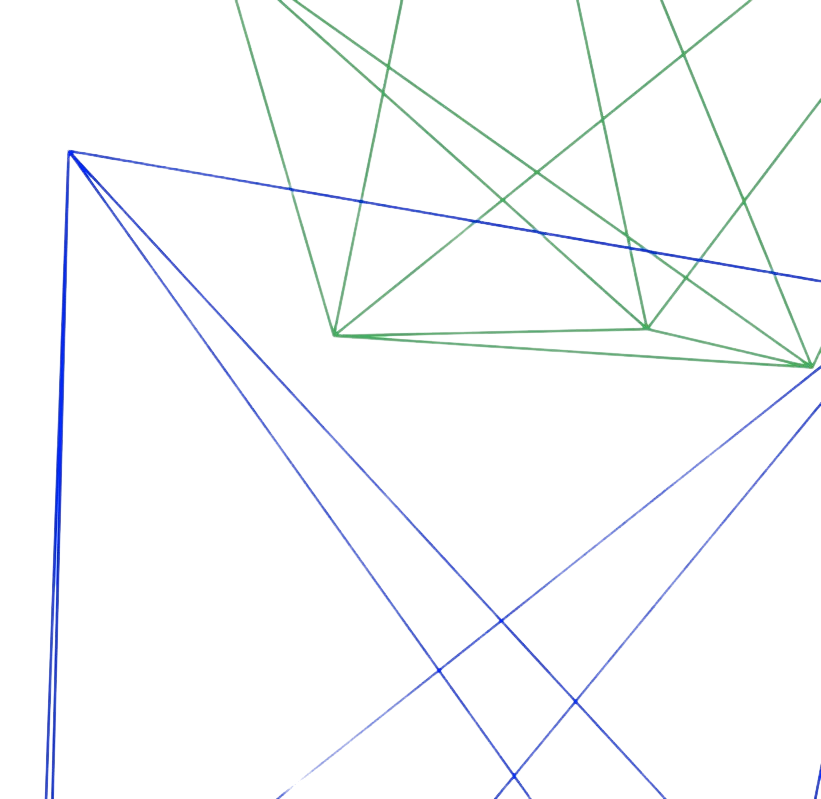
\includegraphics[width=0.5\paperwidth,height=\paperheight]{/root/.config/latex-utils/logos/invert1.png}};

        \node[opacity=0.07,inner sep=0pt, anchor=north west] at (current page.north west){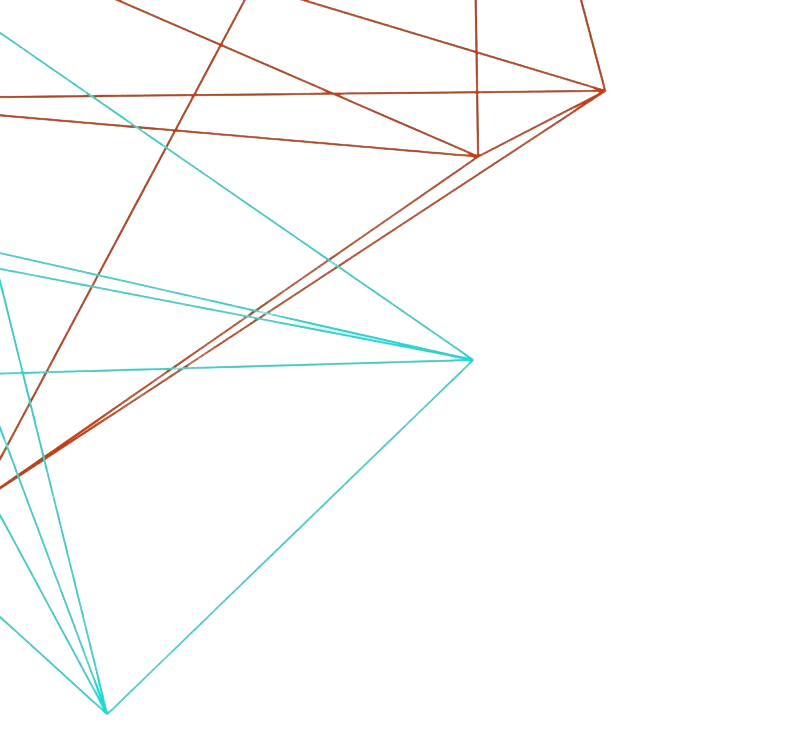
\includegraphics[width=0.5\paperwidth,height=0.5\paperheight]{/root/.config/latex-utils/logos/invert3.png}};




        \node at (page cs:0,0.345) {\Large\textsc{High School Observation and Learning Internship}};
        \node at (page cs:0,0.875) {\Large\bfseries\textsc{Observation Internship}};
        \node at (page cs:0,0.925) {\LARGE\bfseries\textsc{Lycée Français de Barcelone}};

        \node at (page cs:0.5,0) {\Large\textsc{Cyril Lescure - Pedagogical Tutor}};








        %\node[opacity=0.15, inner sep=0pt, anchor=south west] at (current page.south west){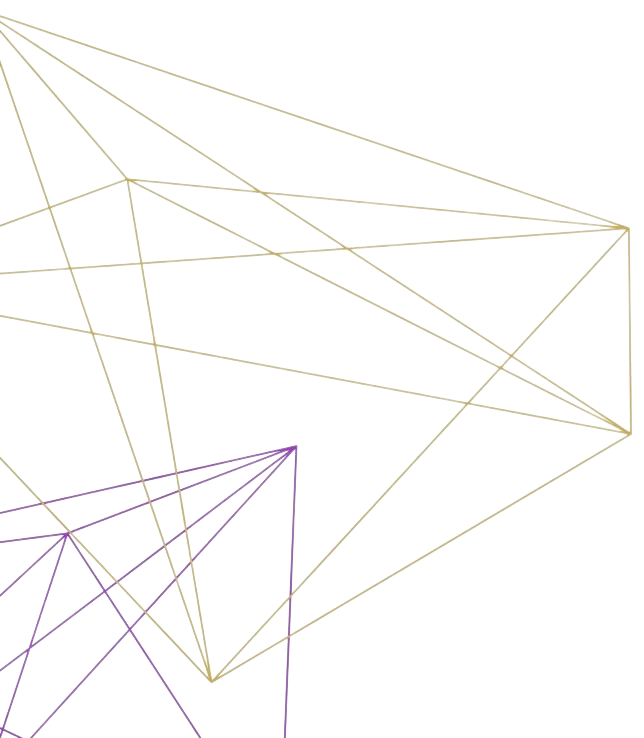
\includegraphics[width=0.5\paperwidth,height=0.5\paperheight]{/root/.config/latex-utils/logos/invert2.png}};

        \node at (page cs:0,0.5) {\fontsize{28}{28.8}\textbf{\ctoptitle}};
        \node at (page cs:0,0.425) {\fontsize{28}{28.8}\textbf{\ctitle}};
        \draw (page cs:0.5,0.375) -- (page cs:-0.5,0.375);
        \node at (page cs:0,0.245) {\LARGE\textsc{\cautor}};
        \node at (page cs:0,0.310) {\Large\textsc{03.06.2019 - 07.06.2019}};


    \end{tikzpicture}
\end{titlepage}


\newgeometry{width=18.625cm, bottom=2cm, top=2cm}

\tikz[remember picture, overlay] \node[opacity=0.3,inner sep=0pt, anchor=north east] at (current page.north east){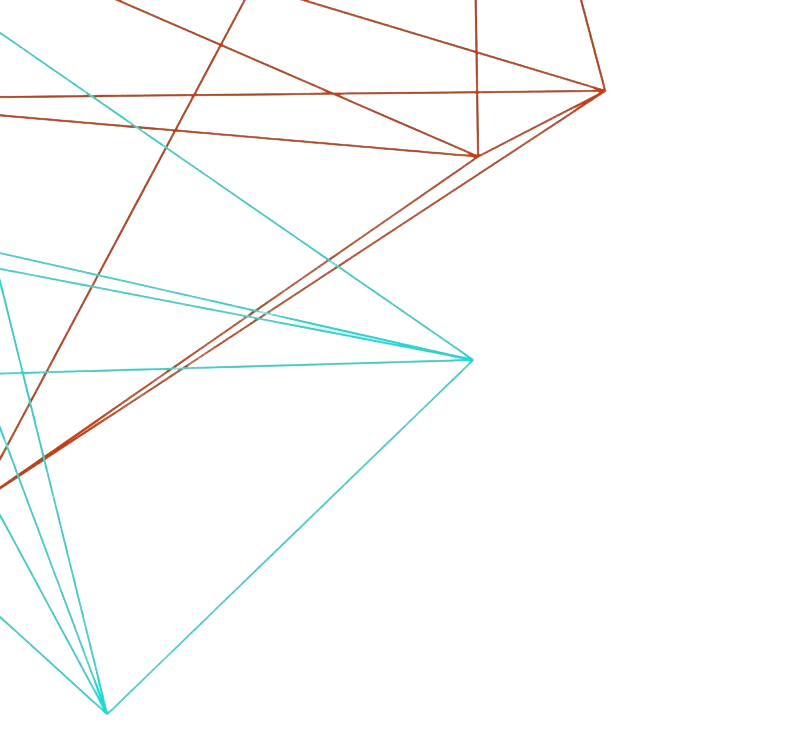
\includegraphics[angle=-90,origin=c,width=0.5\paperheight,height=0.5\paperwidth]{/root/.config/latex-utils/logos/invert3.png}};
\tikz[remember picture,overlay] \node[opacity=0.3,inner sep=0pt, anchor=south east] at (current page.south east){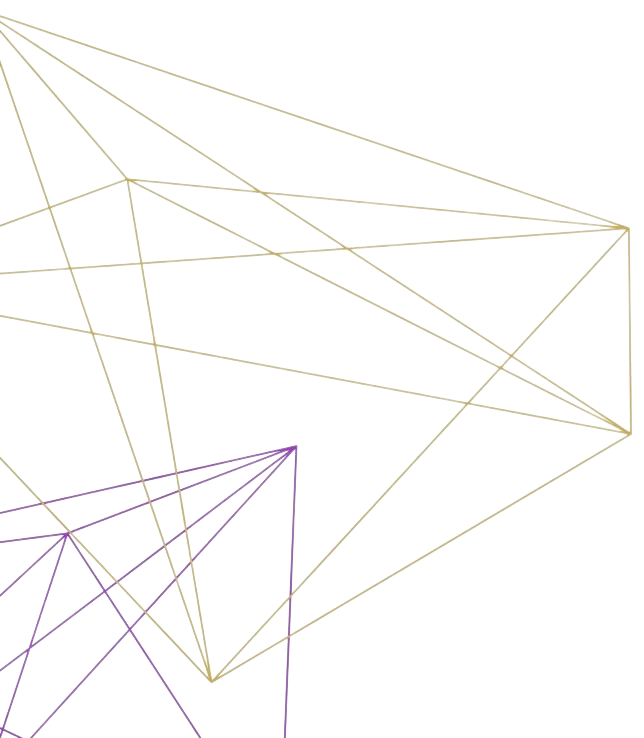
\includegraphics[angle=90,width=0.5\paperwidth,height=0.5\paperheight]{/root/.config/latex-utils/logos/invert2.png}};

\tableofcontents






\newpage


\section{Evaluation de la Transmission Delta}

\subsection{Modulation de Signal}

\subsubsection{Modulateur}
\begin{figure}[ht]
    \begin{floatrow}
        \ffigbox{
            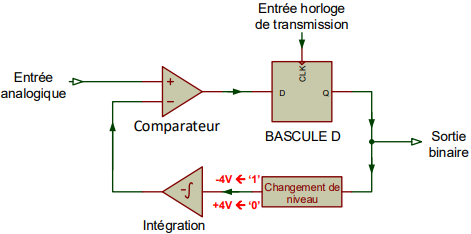
\includegraphics[width=0.55\textwidth]{./object/c1.png}
            \caption{Circuit Modulateur}
        }

        \ffigbox{
            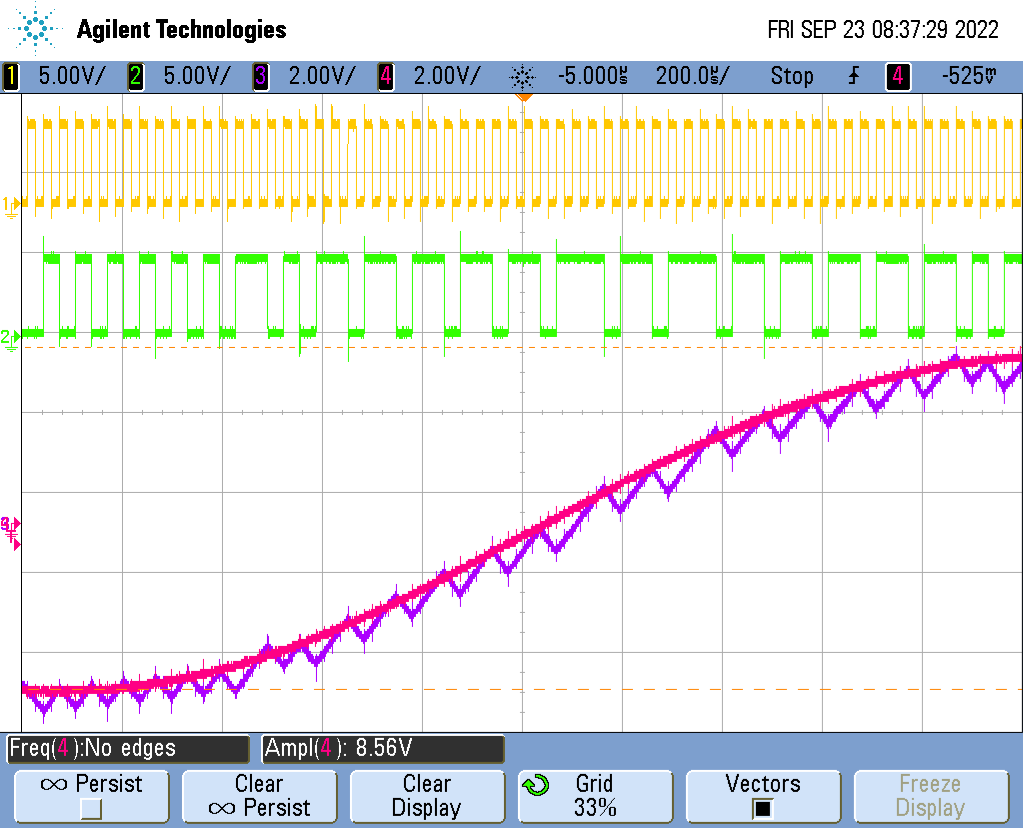
\includegraphics[width=0.35\textwidth]{./object/g1.png}
            \caption{Relevés des chronnogrammes}
        }

    \end{floatrow}
\end{figure}

Sur la carte de développement on construit le circuit du modulateur ci-dessus et pour s'assurer que le circuit fonctionne bien on relève les chronogrammes du \textcolor{green}{\texttt{Data Output}}, du \textcolor{orange}{\texttt{Clock}}, le signal d'entrée \textcolor{pink}{\texttt{Input Signal}} et de la sortie de l'intégrateur \textcolor{purple}{\texttt{Integrator Output}}.

\subsubsection{Démodulateur}

\begin{figure}[ht]
    \begin{floatrow}
        \ffigbox{
            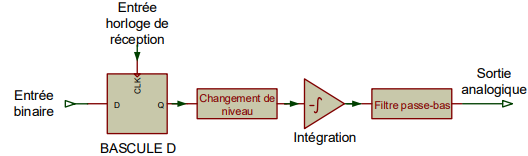
\includegraphics[width=0.55\textwidth]{./object/c2.png}
            \caption{Circuit Démodulateur}
        }

        \ffigbox{
            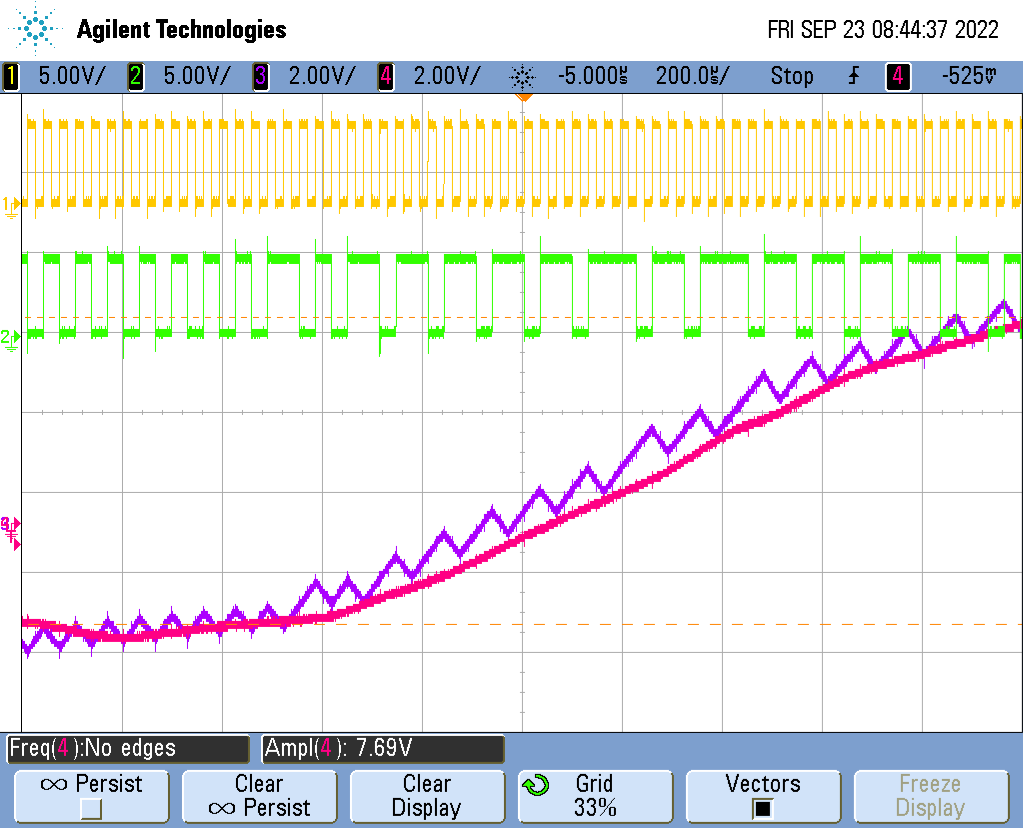
\includegraphics[width=0.35\textwidth]{./object/g2.png}
            \caption{Relevés des chronnogrammes}
        }

    \end{floatrow}
\end{figure}

On construit ensuite le circuit ci-dessus sur la carte de développemment avec l'\textcolor{green}{\texttt{Data Output}} relié à l'entrée binaire \textcolor{green}{\texttt{Data Input}}, et on vérifie que le signal de sortie de la réception \textcolor{pink}{\texttt{Output Signal}} et la \textcolor{orange}{\texttt{Clock}} sont bien branchées et fonctionnent comme il est attendu.

\subsubsection{Observation}

On voit sur le modulateur et le démodulateur le fonctionnement de chacun des ces deux montages.\\
Lorsque l'\textcolor{purple}{\texttt{Integrator Output}} rampe au dessus de l'\textcolor{purple}{\texttt{Input Signal}} le comparateur change l'état de la bascule qui est ensuite synchornisé sur l'horloge en \textcolor{green}{\texttt{Data Output}}. Ce même signal est ensuite démodulé par le circuit inverse, transformant le \textcolor{green}{\texttt{Data Input}} en \textcolor{pink}{\texttt{Output Signal}}.

Cependant lorsque l'on compare l'\textcolor{purple}{\texttt{Input Signal}} avec l'\textcolor{pink}{\texttt{Output Signal}} on s'apercoit d'un légers déphasage entre ces deux signaux.

\begin{figure}[ht!]
    \centering
    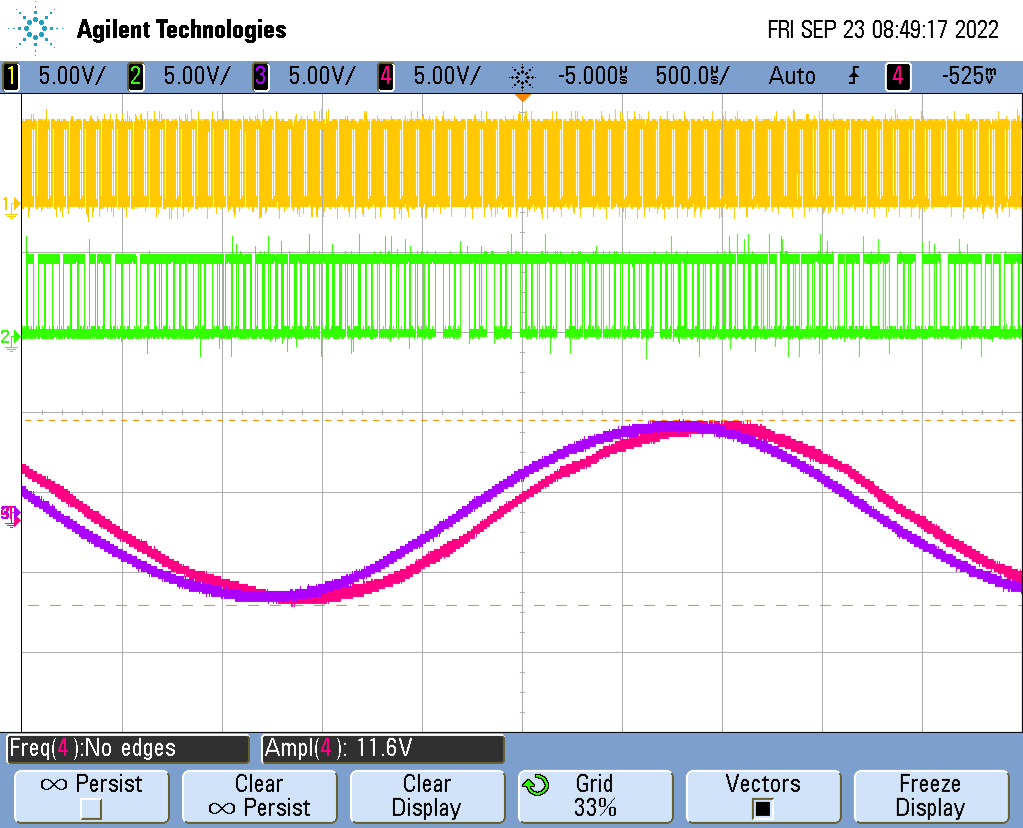
\includegraphics[width=0.4\textwidth]{./object/g3.png}
    \caption{\textcolor{purple}{\texttt{Input Signal}} et \textcolor{pink}{\texttt{Output Signal}}}
\end{figure}

\newpage

Ceci provient du fait que les composants ne sont pas parfait et doivent prendre du temps pour moduler et démoduler les signaux qui leur sont transmis.

\subsection{Étude Caractéristique}
\vspace{-2cm}
\subsubsection{Variation d'Amplitude}
\vspace{-1cm}

Nous verrons comment l'amplitude du signal d'entrée peut modifier le signal qui est modulé. Pour ceci nous règlerons l'\textcolor{purple}{\texttt{Input Signal}} à une fréquence de $\blac 250H_z$ et nous irons varier l'amplitude de $\blac 10$ à $\blac 1V$ pour des fréquences d'horloges chacune plus rapide que l'autre.

\begin{figure}[ht!]
    \centering
    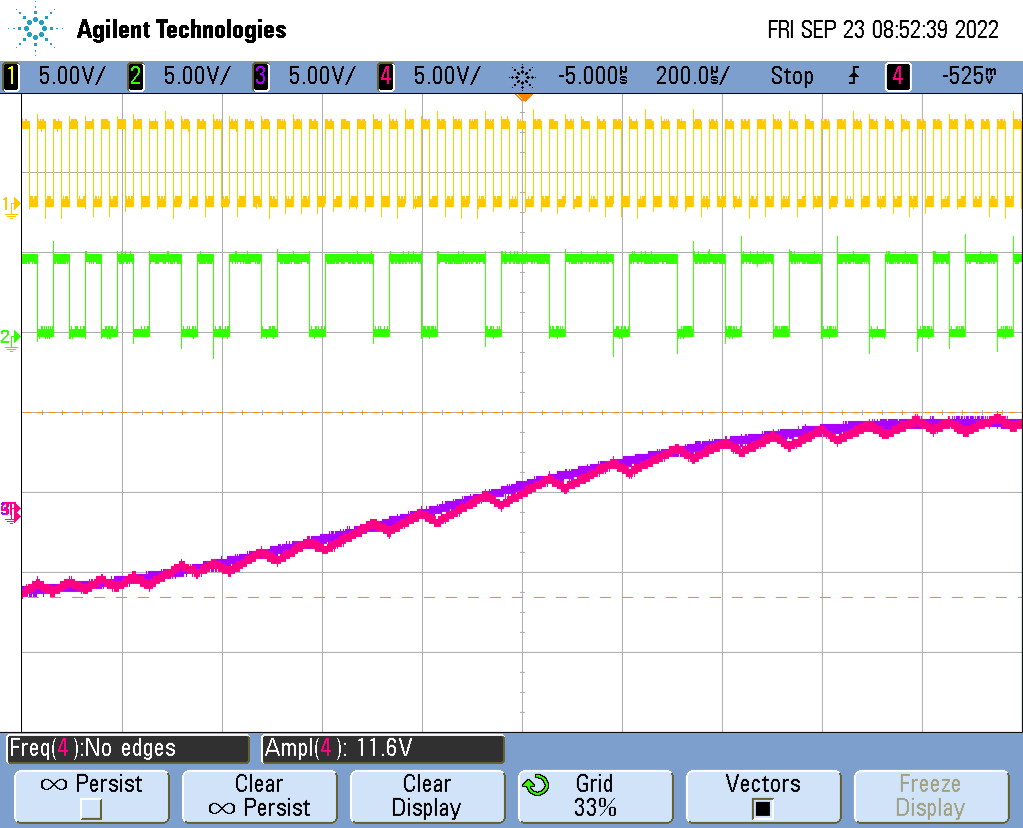
\includegraphics[width=0.4\textwidth]{./object/g4.png}
    \caption{Relevé de référence, $\blac10V$ et $\blac F_{clock}=32kH_z$}
\end{figure}
\begin{center}
    \begin{tabular}{c|c|c}
        Amplitude $V_e$ & $F_{clock}$                  & Observation                                                                                           \\
        \hline
        $10V$           & \multirow{2}{*}{$32\ kH_z$}  & \makecell{On voit qu'en pente l'\textcolor{pink}{\texttt{Integrator Output}} met un peu de temps pour \\ atteindre  l'\textcolor{purple}{\texttt{Input Signal}} mais suis correctement ce\\ dernier.}\\
        \cline{1-1}\cline{3-3}
        $1V$            &                              & \makecell{On observe que l'\textcolor{pink}{\texttt{Integrator Output}} forme un signal de            \\ rampe mais qui monte et descend en escalier}\\
        \hline
        $10V$           & \multirow{2}{*}{$64\ kH_z$}  & \makecell{On observe que l'\textcolor{pink}{\texttt{Integrator Output}} suit mieux le                 \\ signal d’entrée.}\\
        \cline{1-1}\cline{3-3}
        $1V$            &                              & \makecell{On observe que l'\textcolor{pink}{\texttt{Integrator Output}} forme toujours                \\ un signal qui monte en escalier, mais ils y des paliers\\ plus nombreux}\\
        \hline
        $10V$           & \multirow{2}{*}{$128\ kH_z$} & \makecell{On observe que l'\textcolor{pink}{\texttt{Integrator Output}} suit bien                     \\ mieux le signal d’entrée, le \textcolor{green}{\texttt{Data Output}} varie plus.}\\
        \cline{1-1}\cline{3-3}
        $1V$            &                              & \makecell{On observe que l'\textcolor{pink}{\texttt{Integrator Output}} forme toujours                \\ un signal qui monte en escalier, et on a des paliers\\ de plus en plus nombreux}\\
        \hline
        $10V$           & \multirow{2}{*}{$256\ kH_z$} & \makecell{On observe que l'\textcolor{pink}{\texttt{Integrator Output}} suit presque                  \\ parfaitement l'\textcolor{purple}{\texttt{Input Signal}}, le \textcolor{green}{\texttt{Data Output}} \\varie beaucoup plus.}\\
        \cline{1-1}\cline{3-3}
        $1V$            &                              & \makecell{On observe que l'\textcolor{pink}{\texttt{Integrator Output}} ne forme presque plus         \\de paliers}\\
    \end{tabular}
\end{center}

\begin{dent}{Déductions:} On voit que pour des amplitudes petites, l'intégrateur est trop rapide et le signal d'horloge trop lent, la sortie de la bascule "lag" face à son entrée. De ce fait on observe un signal de rampe qui fait des paliers et ne module pas fidèlement le signal d'entrée.

    En influenceant directement sur la rapiditée de l'horloge, on augmente la rapidité de la bascule ce qui néglige le delai ressenti entre son entrée et sa sortie. On remarque ainsi que la taille des paliers réduit considérablement, permetant ainsi au signal intégrateur de suivre plus proprement l'entrée.

    Sur des signaux à haute amplitude cet effet est moins ressenti puisque l'amplitude du signal d'entrée est suffisemment grande donc il doit y avoir plus de paliers pour traiter le signal.

    Cependant il y a un contre-effet auquel il faut faire attention; si le signal d'entrée posède une amplitude trop grande, sa pente augementera, et de ce fait il est possible que la pente du signal d'entrée soit supérieur à celle de l'intégrateur, il y aura donc saturation de la pente.

\end{dent}

\subsubsection{Variation en Fréquence}

\vspace{-3cm}

Maintenant que nous ayons vu les effets que peut donner l'amplitude du signal d'entrée, nous nous intéresserons au effet ressenti lorsque l'on modifie sa fréquence.

\begin{center}
    \begin{tabular}{c|c|c}
        Fréquence de $V_e$         & $F_{clock}$ & Observation                                                                                    \\
        \hline
        \multirow{2}{*}{$250H_z$}  & $32\ kH_z$  & \makecell{Il n’y a pas de saturation de la pente et la modulation du signal est faible}        \\
        \cline{2-3}
                                   & $256\ kH_z$ & \makecell{Il n’y a pas de saturation de la pente et la modulation du signal est fort}          \\
        \hline
        \multirow{2}{*}{$500H_z$}  & $32\ kH_z$  & \makecell{On commence à observer une saturation de la pente et la modulation                   \\ du signal reste faible}\\
        \cline{2-3}
                                   & $256\ kH_z$ & \makecell{On observe une saturation de la pente cependant                                      \\ la modulation du signal reste fort ce qui permet de suivre\\ l'\textcolor{purple}{\texttt{Input Signal}} (chronogramme 1)} \\
        \hline
        \multirow{2}{*}{$1\ kH_z$} & $32\ kH_z$  & \makecell{La pente de l'\textcolor{pink}{\texttt{Integrator Output}} n'est pas assé forte      \\ pour suivre l'\textcolor{purple}{\texttt{Input Signal}}, on voit\\ donc un signal triangulaire}\\
        \cline{2-3}
                                   & $256\ kH_z$ & \makecell{La pente de l'\textcolor{pink}{\texttt{Integrator Output}} n'est pas assé forte      \\ pour correctement suivre l'\textcolor{purple}{\texttt{Input Signal}}, on voit\\ donc un signal triangulaire (chronogramme 2)} \\
        \hline
        \multirow{2}{*}{$2\ kH_z$} & $32\ kH_z$  & \makecell{La pente de l'\textcolor{pink}{\texttt{Integrator Output}} n'est pas assé forte      \\ pour suivre l'\textcolor{purple}{\texttt{Input Signal}}, on voit\\ donc un signal triangulaire qui à réduit d'amplitude}\\
        \cline{2-3}
                                   & $256\ kH_z$ & \makecell{La pente de l'\textcolor{pink}{\texttt{Integrator Output}} n'est pas assé forte pour \\correctement suivre l'\textcolor{purple}{\texttt{Input Signal}}, on voit donc un signal \\triangulaire qui à réduit d'amplitude (chronogramme 3)} \\
    \end{tabular}
\end{center}

\begin{figure}[ht!]
    \centering
    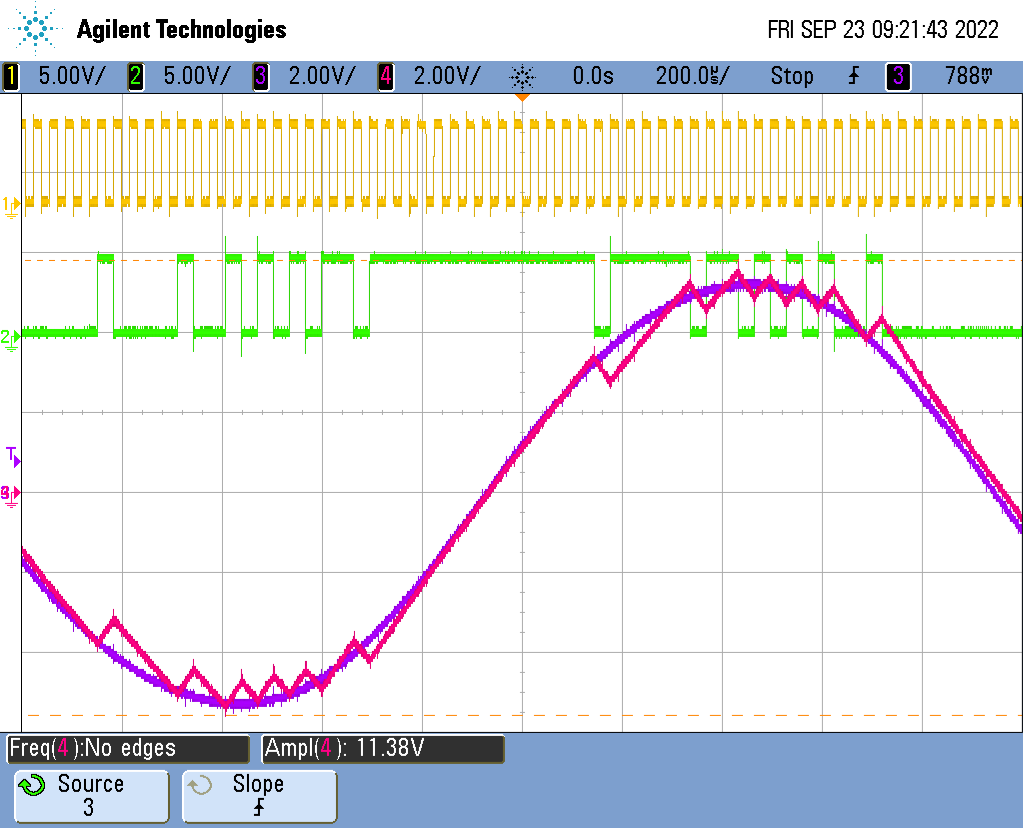
\includegraphics[width=0.32\textwidth]{./object/g5.png}
    \hspace{0.05\textwidth}
    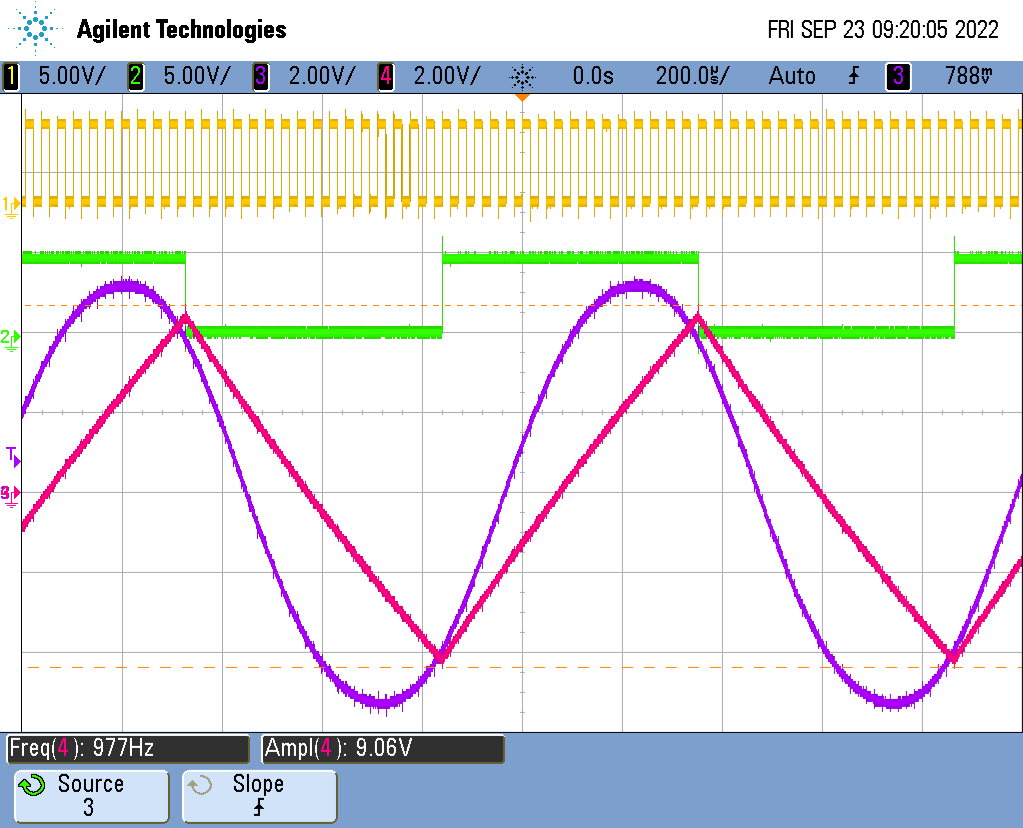
\includegraphics[width=0.32\textwidth]{./object/g6.png}
    \hspace{0.05\textwidth}
    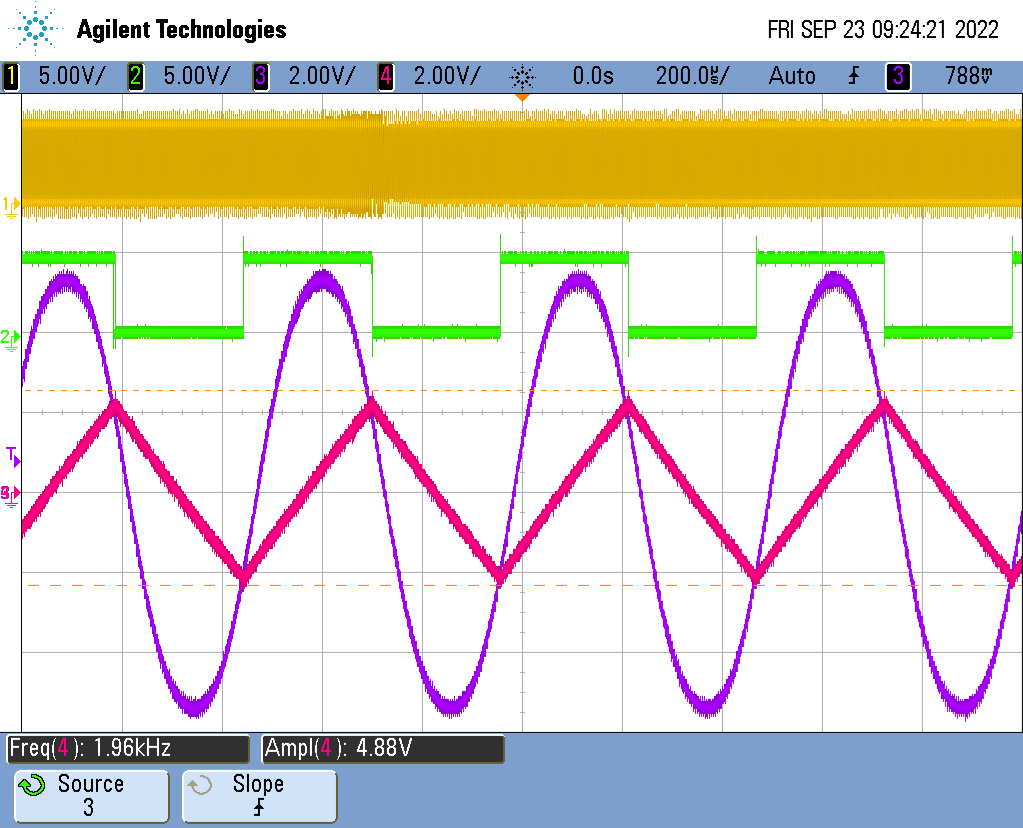
\includegraphics[width=0.32\textwidth]{./object/g7.png}
    \caption{Chronogrammes 1, 2 et 3}
\end{figure}



\begin{dent}{Déduction:} En augmentant la fréquence du signal d'entrée on augmente aussi la pente de ce signal. Il arrive donc un point où la pente du signal est supérieure à celle de l'intégrateur, il y a saturation de la pente.\\

    Modifier la vitesse de l'horloge ne permet pas de compenser cet effet puisque le problème vient du fait que l'intégrateur ne peut pas ratrapper le signal d'entrée, et l'horloge ne peut pas modifier ceci.\\

    Lorsqu'il y a sursaturation de la pente on finit donc par observer une signal qui apparait triangulaire et ne module pas proprement le signal d'entrée. Le modulateur renvoi un donc un signal triangulaire.
\end{dent}



\subsection{Étude en Amplification}

On intervient maintenant le \texttt{Gain Control} de l'intégrateur pour expliquer les effets d'une amplification sur la qualité de la transmission.

En utilisant les curseurs verticaux sur l'oscilloscope nous allons mesurer le temps que mets la rampe pour aller d'un pic à l'autre, et en utilisant les curseurs horizontaux nous mesurerons la variation de tension entre ces deux pics. \\
On obtient ainsi le temps que mets la rampe pour monter de $\delta x$ volts.

On mesure ainsi les données suivantes:

\begin{center}
    \begin{tabular}{c|c|c|c}
        AB & Pente            & AB & Pente            \\
        \hline
        00 & $0.02\ V/\mu s$  & 10 & $0.07\ V/\mu s$  \\
        \hline
        01 & $0.034\ V/\mu s$ & 11 & $0.137\ V/\mu s$
    \end{tabular}
\end{center}

On regarde ensuite le comportement des signaux lorsque ce gain est modifié. En premier lieu avec un signal d'entrée à $250H_z$ et en deuxième lieu avec une fréquence de $2\ kH_z$.

\subsubsection{Fréquence faible}

\begin{center}
    \begin{tabular}{c|c|c}
        Gain Control        & $F_{clock}$ & Observation                                                                 \\
        \hline
        \multirow{2}{*}{00} & $32\ kH_z$  & \makecell{La courbe n’est pas saturée, la modulation est faible             \\ et elle suit la courbe du signal d’entrée (chronogramme 1)}\\
        \cline{2-3}
                            & $256\ kH_z$ & \makecell{La courbe n’est pas saturée, on remarque l'apparition de paliers, \\ la modulation est forte et elle suit mieux la courbe\\ du signal d’entrée}\\
        \hline
        \multirow{2}{*}{01} & $32\ kH_z$  & \makecell{On observe que la pente de l'intégrateur est plus élevée.         \\ On commence à retrouver des paliers}\\
        \cline{2-3}
                            & $256\ kH_z$ & \makecell{La courbe n’est pas saturée, la modulation est forte et           \\ elle suit mieux la courbe du signal d’entrée\\ et on voit moins les paliers}\\
        \hline
        \multirow{2}{*}{10} & $32\ kH_z$  & \makecell{La modulation est faible, on voit que les paliers sont très       \\ prononcés, la sortie de l'intégrateur à du mal à suivre le\\ signal d'entrée (chronogramme 2)}\\
        \cline{2-3}
                            & $256\ kH_z$ & \makecell{On ne voit plus du tout de paliers, la sortie de l'intégrateur    \\ suit le signal d'entrée} \\
        \hline
        \multirow{2}{*}{11} & $32\ kH_z$  & \makecell{La modulation est faible, on voit que les paliers sont très       \\ prononcés, la sortie de l'intégrateur à du mal à suivre\\ le signal d'entrée (chronogramme 3)}\\
        \cline{2-3}
                            & $256\ kH_z$ & \makecell{On retrouve les paliers mais la forte modulation permet de        \\ compenser cet effet ainsi la sortie de l’intégrateur suit\\ le signal d’entrée.} \\
    \end{tabular}
\end{center}

\begin{figure}[ht]
    \centering
    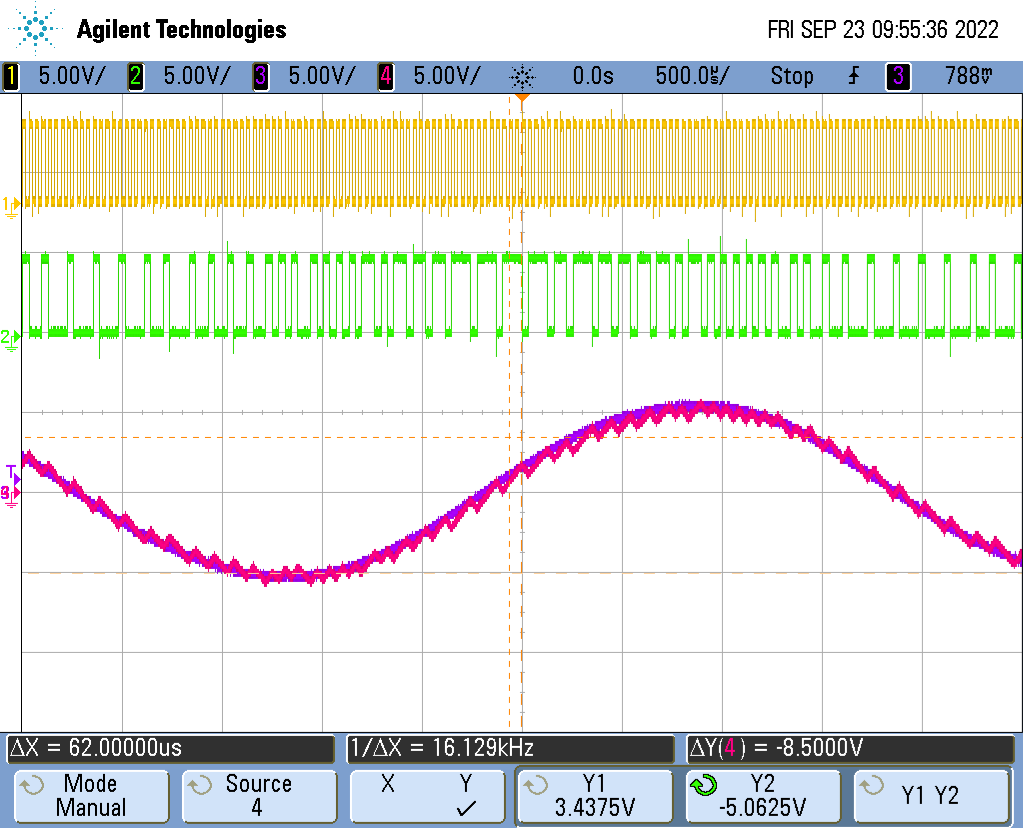
\includegraphics[width=0.45\textwidth]{./object/g8.png}
    \hspace{0.05\textwidth}
    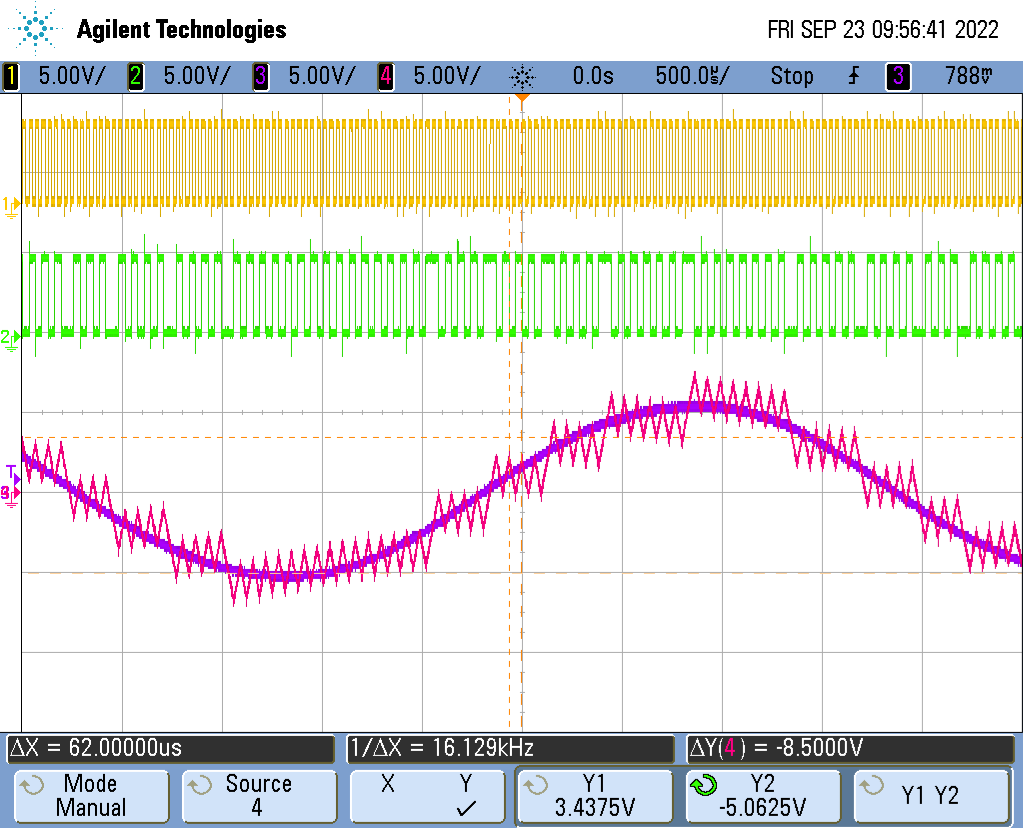
\includegraphics[width=0.45\textwidth]{./object/g9.png}
    \hspace{0.05\textwidth}
    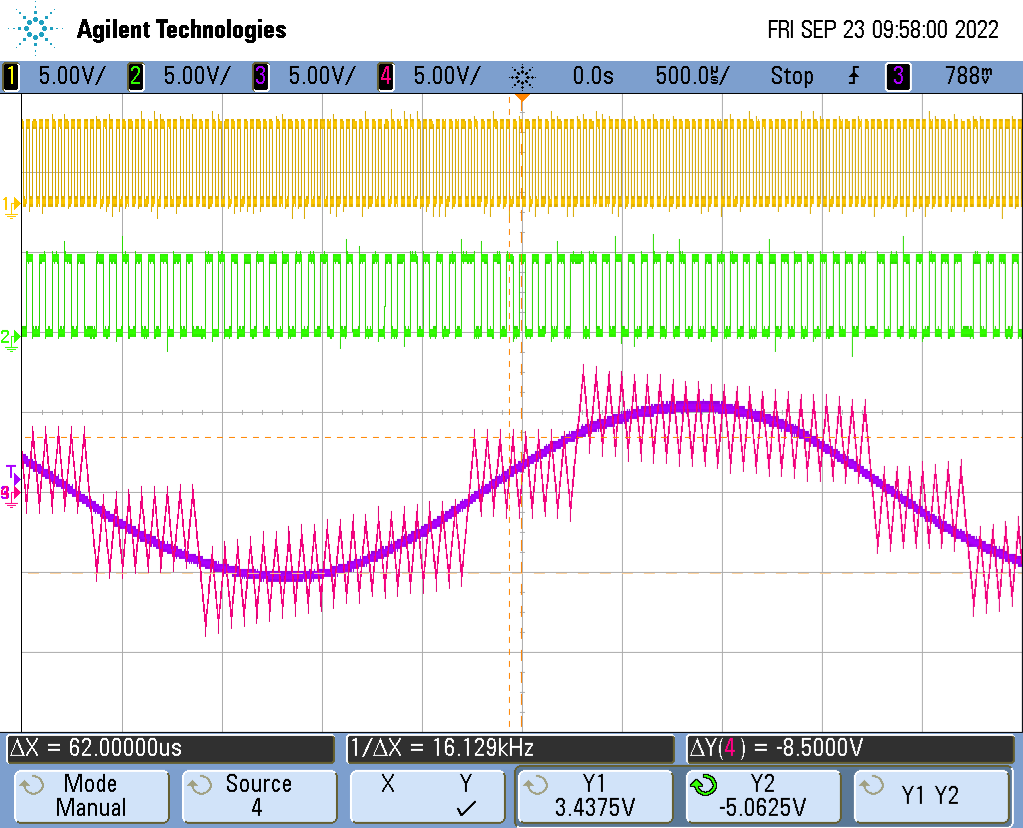
\includegraphics[width=0.45\textwidth]{./object/g10.png}
    \caption{Chronogrammes 1, 2 et 3}
\end{figure}

\newpage

\subsubsection{Fréquence Haute}

\begin{center}
    \begin{tabular}{c|c|c}
        Gain Control        & $F_{clock}$ & Observation                                                                \\
        \hline
        \multirow{2}{*}{00} & $32\ kH_z$  & \makecell{Le signal de la sortie de l’intégrateur est triangulaire         \\ avec une amplitude faible, il n’arrive pas à suivre\\ le signal d’entrée. (Chronogramme 1)}\\
        \cline{2-3}
                            & $256\ kH_z$ & \makecell{Le signal de la sortie de l’intégrateur est triangulaire avec    \\ une amplitude faible, il n’arrive pas à suivre le signal d’entrée.}\\
        \hline
        \multirow{2}{*}{01} & $32\ kH_z$  & \makecell{Le signal de la sortie de l’intégrateur est triangulaire         \\ avec une amplitude plus élevée, il n’arrive pas à\\ suivre le signal d’entrée.}\\
        \cline{2-3}
                            & $256\ kH_z$ & \makecell{Le signal de la sortie de l’intégrateur est triangulaire avec    \\ une amplitude plus élevée, il n’arrive pas à suivre le signal d’entrée.}\\
        \hline
        \multirow{2}{*}{10} & $32\ kH_z$  & \makecell{Le signal de la sortie de l’intégrateur commence à suivre le     \\ signal d’entrée, il reste encore triangulaire. (Chronogramme 2) }\\
        \cline{2-3}
                            & $256\ kH_z$ & \makecell{Le signal de la sortie de l’intégrateur suit le signal d’entrée, \\ on observe une saturation de la pente. (Chronogramme 3)} \\
        \hline
        \multirow{2}{*}{11} & $32\ kH_z$  & \makecell{Le signal de la sortie de l’intégrateur suit le signal           \\ d’entrée mais il reste très triangulaire du fait de\\ sa faible fréquence . (Chronogramme 4)}\\
        \cline{2-3}
                            & $256\ kH_z$ & \makecell{Le signal de la sortie de l’intégrateur suit de très             \\ près le signal d’entrée et il n’y a pas\\ de saturation de la pente. (Chronogramme 5)} \\
    \end{tabular}
\end{center}


\begin{figure}[ht!]
    \centering
    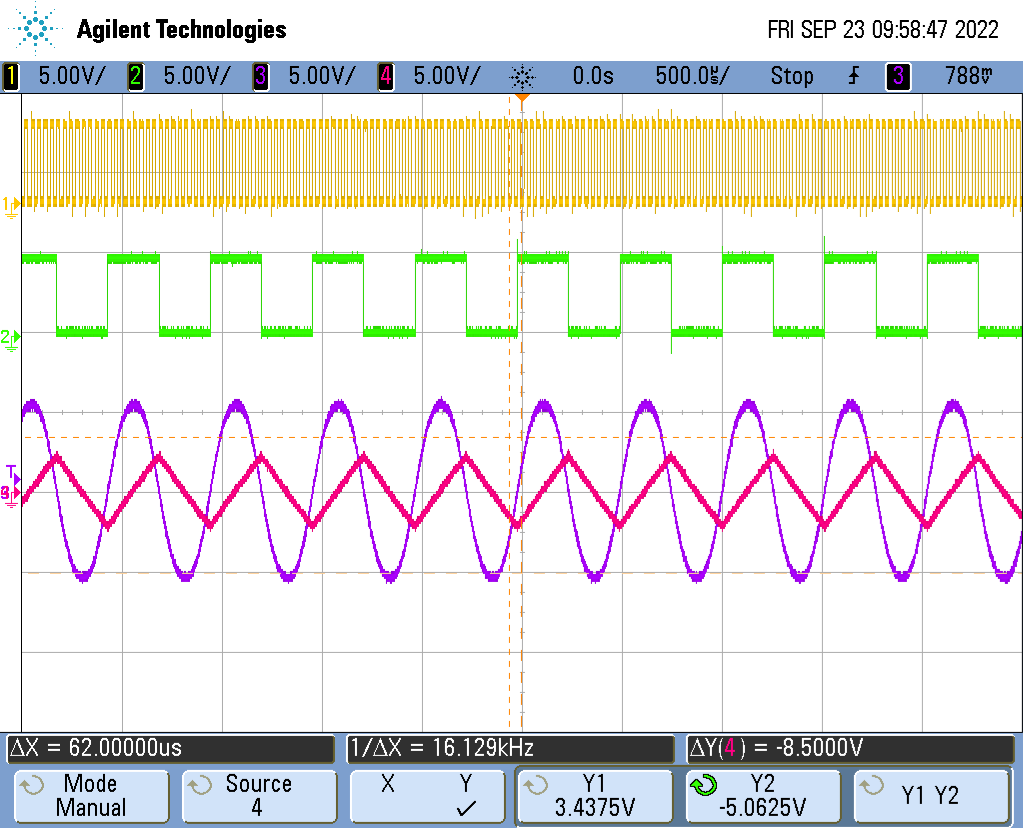
\includegraphics[width=0.3\textwidth]{./object/g11.png}
    \hspace{0.05\textwidth}
    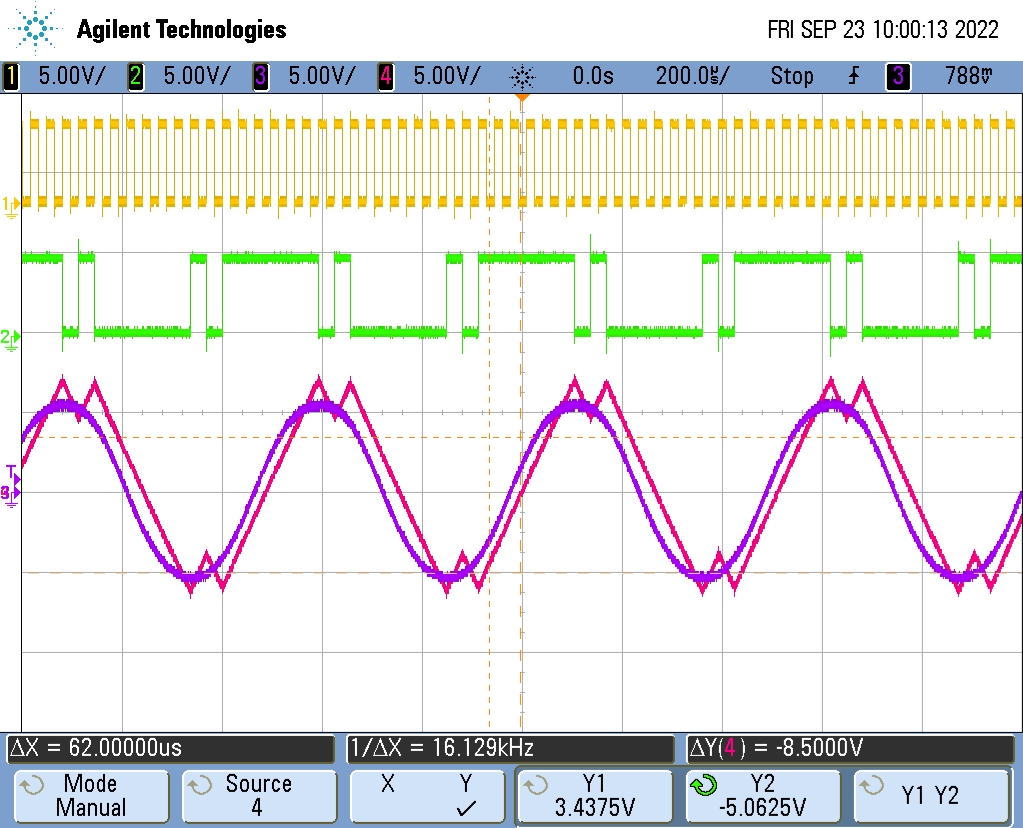
\includegraphics[width=0.3\textwidth]{./object/g12.png}
    \hspace{0.05\textwidth}
    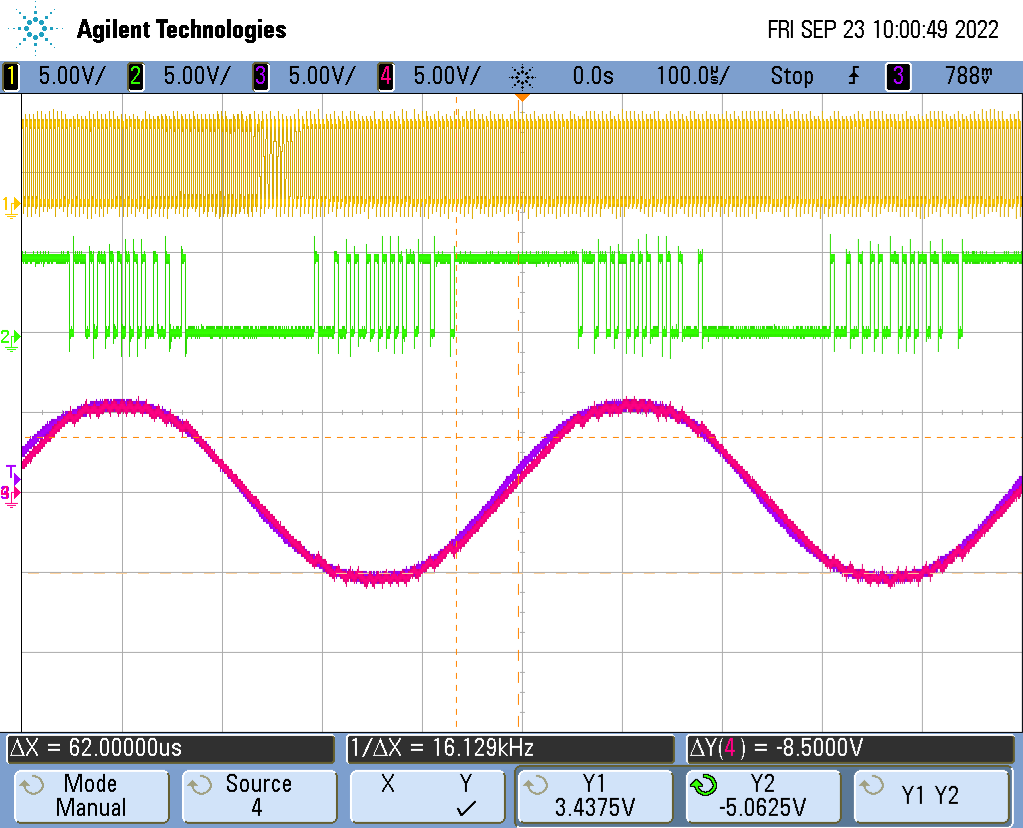
\includegraphics[width=0.3\textwidth]{./object/g13.png}
    \hspace{0.05\textwidth}
    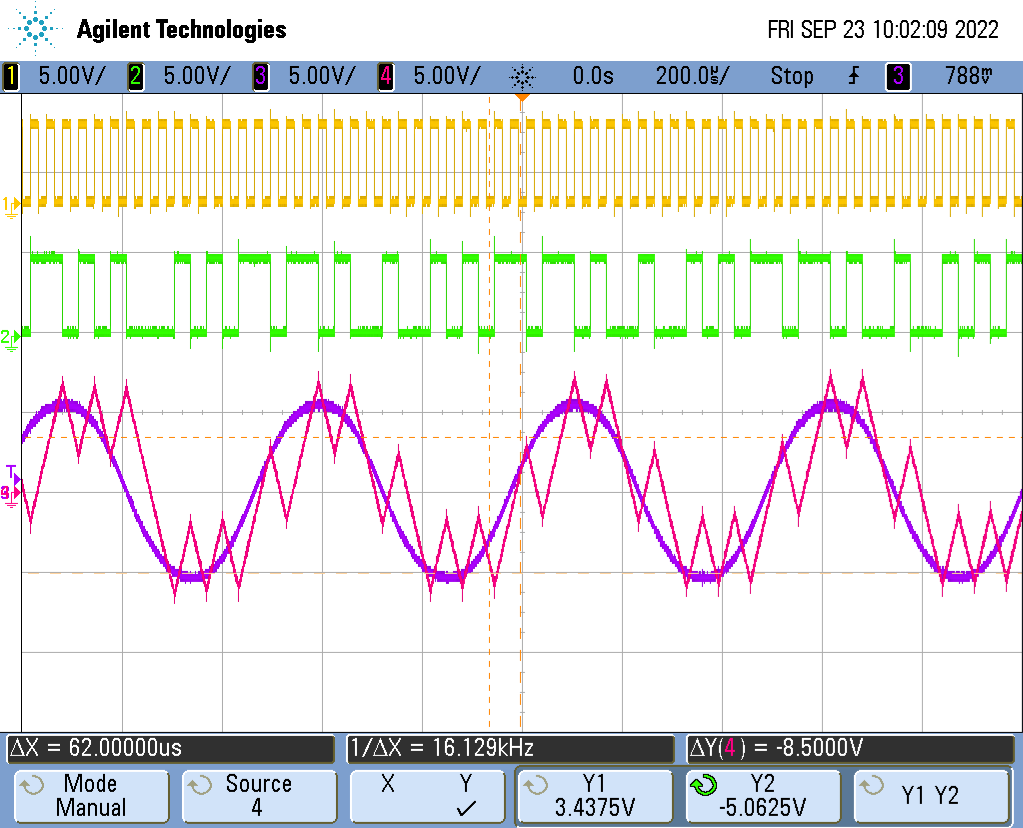
\includegraphics[width=0.3\textwidth]{./object/g14.png}
    \hspace{0.05\textwidth}
    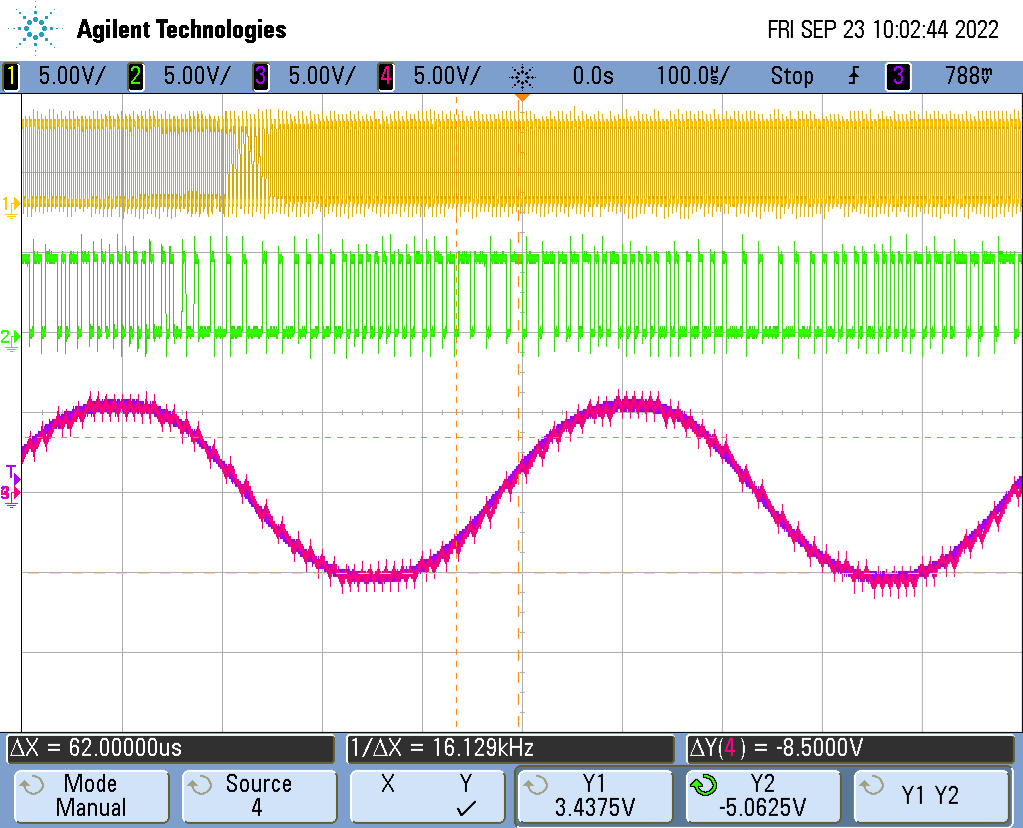
\includegraphics[width=0.3\textwidth]{./object/g15.png}
    \caption{Chronogrammes 1, 2, 3, 4, et 5}
\end{figure}

\newpage

\begin{dent}{Déduction:}En augmentant le gain on augmente aussi la pente de l'intégrateur. Comme nous pouvions le voir il est donc utile d'avoir un gain élevé en haute fréquence pour que l'intégrateur puisse correctement suivre
    le signal d'entrée. \\

    Ceci ne nous aide pas par contre lorsque nous sommes sur des faibles fréquences, on commence à retrouver des paliers.
\end{dent}

\section{Modulation Delta Adaptive}

\begin{figure}[ht!]
    \begin{floatrow}
        \ffigbox{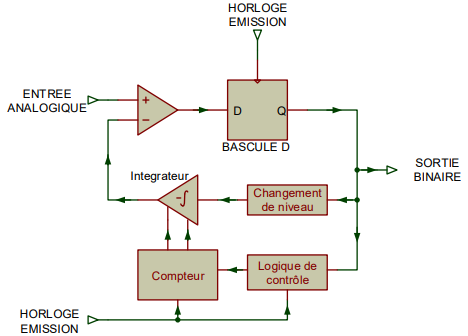
\includegraphics[width=0.32\textwidth]{./object/c3.png}\caption{Circuit de la modulation adaptive}}

        \ffigbox{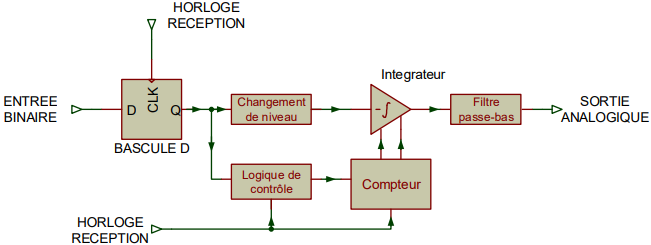
\includegraphics[width=0.32\textwidth]{./object/c4.png}\caption{Circuit de la démodulation adaptive}}

    \end{floatrow}
\end{figure}

\begin{figure}[ht!]
    \begin{floatrow}
        \ffigbox{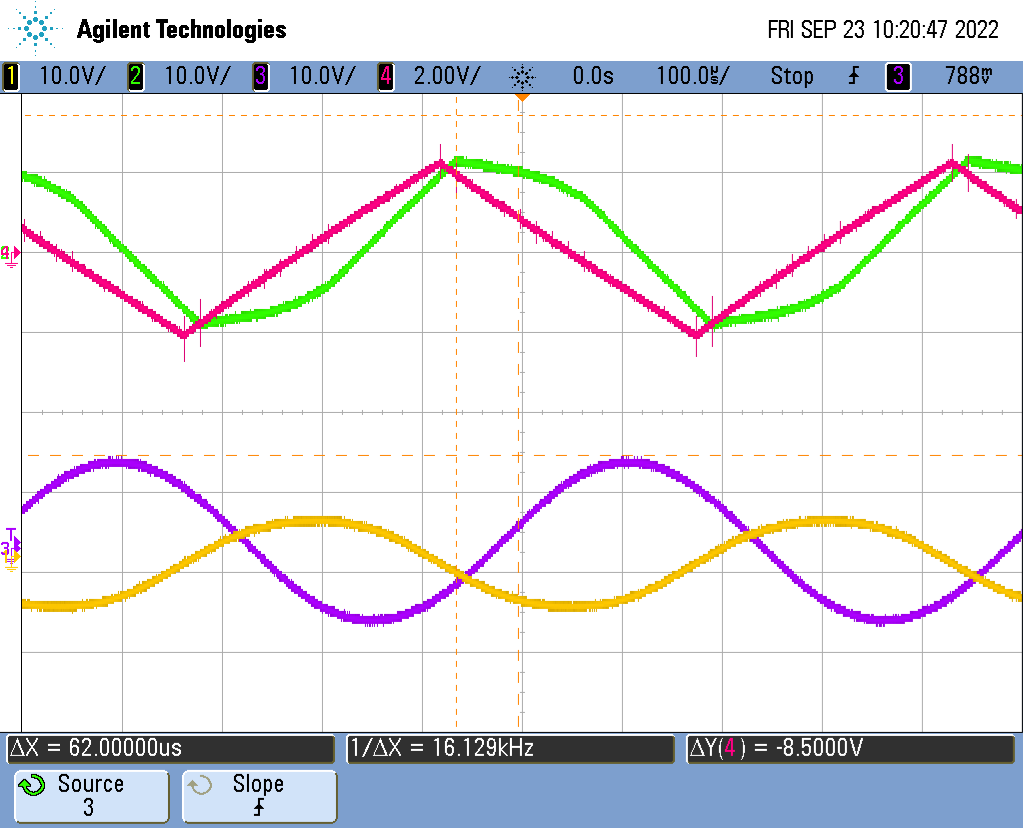
\includegraphics[width=0.32\textwidth]{./object/g16.png}\caption{Entrées et sorties, $32\ kH_z$}}

        \ffigbox{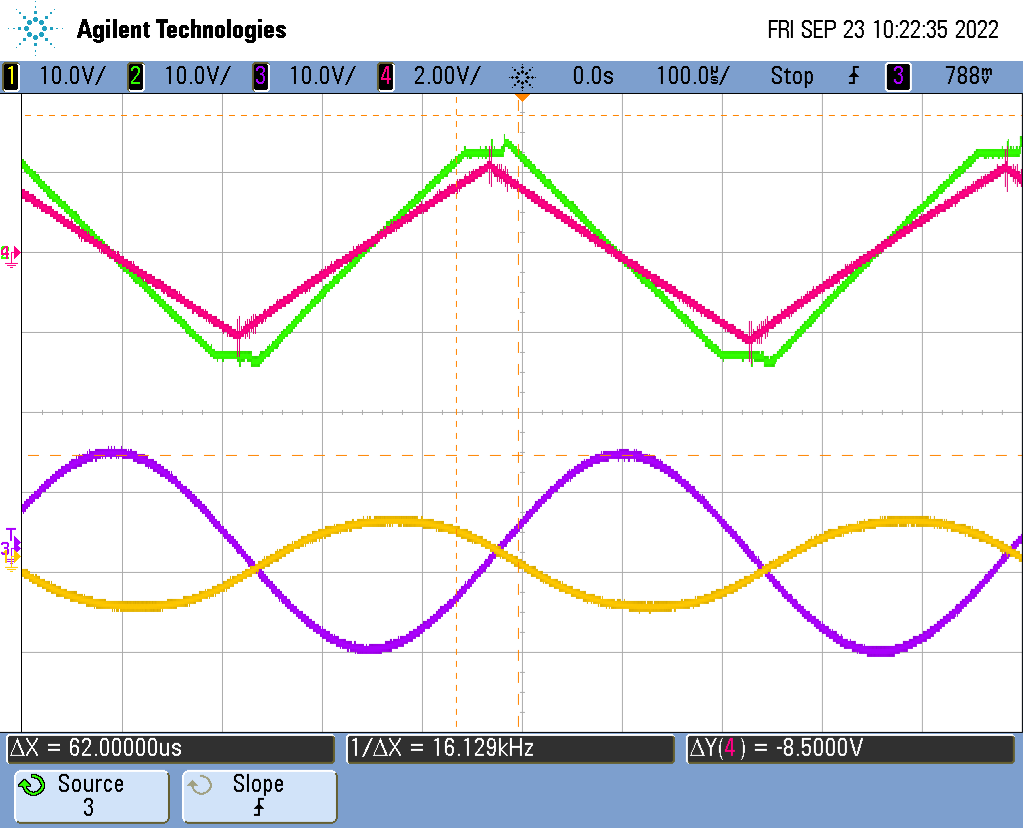
\includegraphics[width=0.32\textwidth]{./object/g17.png}\caption{Entrées et sorties, $256\ kH_z$}}

    \end{floatrow}
\end{figure}

\begin{dent}{Déduction :} On voit que pour une fréquence d'entrée à $2\ kH_z$ le modulateur envoi un signal triangulaire à la \textcolor{pink}{sortie de son intégrateur} qui ne correspond pas correctement au \textcolor{orange}{signal d'entrée}.

    Ceci est ensuite transmis au démodulateur avec une signal déformé a la \textcolor{green}{sortie de son intégrateur} donnant un \textcolor{purple}{signal de sortie} qui ne correspond pas tout à fait au \textcolor{orange}{signal d'entrée}, il est légèrement amplifié et déphasé.

    Comme nous avions vu précédemment l'horloge n'influence pas la qualité de transmission lorsque le signal d'entrée est à de hautes fréquences, donc le \textcolor{purple}{signal de sortie} ressemble fortement dans les deux cas.
\end{dent}

En mettant ensuite les deux gains controllés par le compteur on obtient le signal suivant:

\begin{figure}[ht]
    \centering
    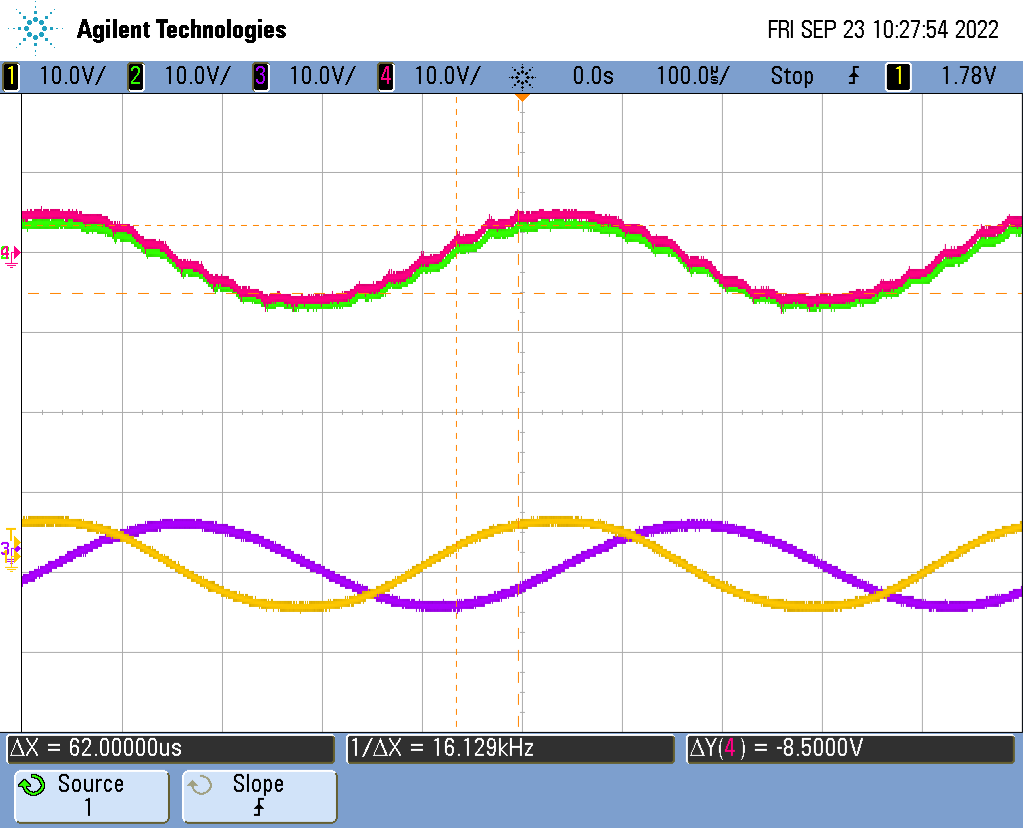
\includegraphics[width=0.55\textwidth]{./object/g18.png}
\end{figure}

Cette fois-ci on voit bien que les entrées et les sorties du modulateur et démodulateur se ressemblent fortement l'un l'autre

\subsection{Conclusion}

Nous venons donc de voir plusieurs méthodes différentes de moduler un signal. Soit par modulation delta simple, ou par modulation delta adaptive.

On a vu que la modulation delta simple s'effectuait en règlant le gain de l'intégrateur et en augmentant la vitesse de l'horloge. Cependant pour que la transmission puisse fonctionner correctement il faut que ces deux paramètres soit aussi passées au démodulateur.

La modulation delta adaptive permet d'eliminer ce souci en partageant une même horloge qui à la foit permet de controler simultanément le gain du modulateur et démodulateur. De cette manière la transmission est correctement transmise.


\end{document}